% !TeX root = main.tex

\chapter{Huffman Encoding}
\glsresetall
\label{chapter:huffman}

\section{Background}

Lossless data compression is a key ingredient for efficient data storage, and Huffman coding is amongst the most popular algorithms for variable length coding \cite{huffman1952method}. Given a set of data symbols and their frequencies of occurrence, Huffman coding generates codewords in a way that assigns shorter codes to more frequent symbols to minimize the average code length. Since it guarantees optimality, Huffman coding has been widely adopted for various applications \cite{flannery1992numerical}. In modern multi-stage compression designs, it often functions as a back-end of the system to boost compression performance after a domain-specific front-end as in GZIP \cite{deutsch1996deflate}, JPEG \cite{pennebaker1992jpeg}, and MP3 \cite{sherigar2004huffman}. Although arithmetic encoding \cite{witten1987arithmetic}  (a generalized version of Huffman encoding which translates an entire message into a single number) can achieve better compression for most scenarios, Huffman coding has often been the algorithm of choice for many systems because of patent concerns with arithmetic encoding \cite{langdon1990arithmetic}.

Canonical Huffman coding has two main benefits over traditional Huffman coding. In basic Huffman coding, the encoder passes the complete Huffman tree structure to the decoder. Therefore, the decoder must traverse the tree to decode every encoded symbol. On the other hand, canonical Huffman coding only transfers the number of bits for each symbol to the decoder, and the decoder reconstructs the codeword for each symbol. This makes the decoder more efficient both in memory usage and computation requirements. Thus, we focus on canonical Huffman coding.

In basic Huffman coding, the decoder decompresses the data by traversing the Huffman tree from the root until it hits the leaf node. This has two major drawbacks: it requires storing the entire Huffman tree which increases memory usage. Furthermore, traversing the tree for each symbol is computationally expensive. Canonical Huffman encoding addresses these two issues by creating codes using a standardized canonical format.  The benefit of using a canonical encoding is that we only need to transmit the length of each Huffman codeword.  A Canonical Huffman code has two additional properties.  Firstly, longer length codes have a higher numeric value than the same length prefix of shorter codes.  Secondly, codes with the same length increase by one as the symbol value increases. This means if we know the starting symbol for each code length, we can easily reconstruct the canonical Huffman code.  The Huffman tree is essentially equivalent to a `sorted' version of the original Huffman tree so that longer codewords are on the right-most branch of the tree and all of the nodes at the same level of the tree are sorted in order of the symbols.  

\begin{figure}
\centering
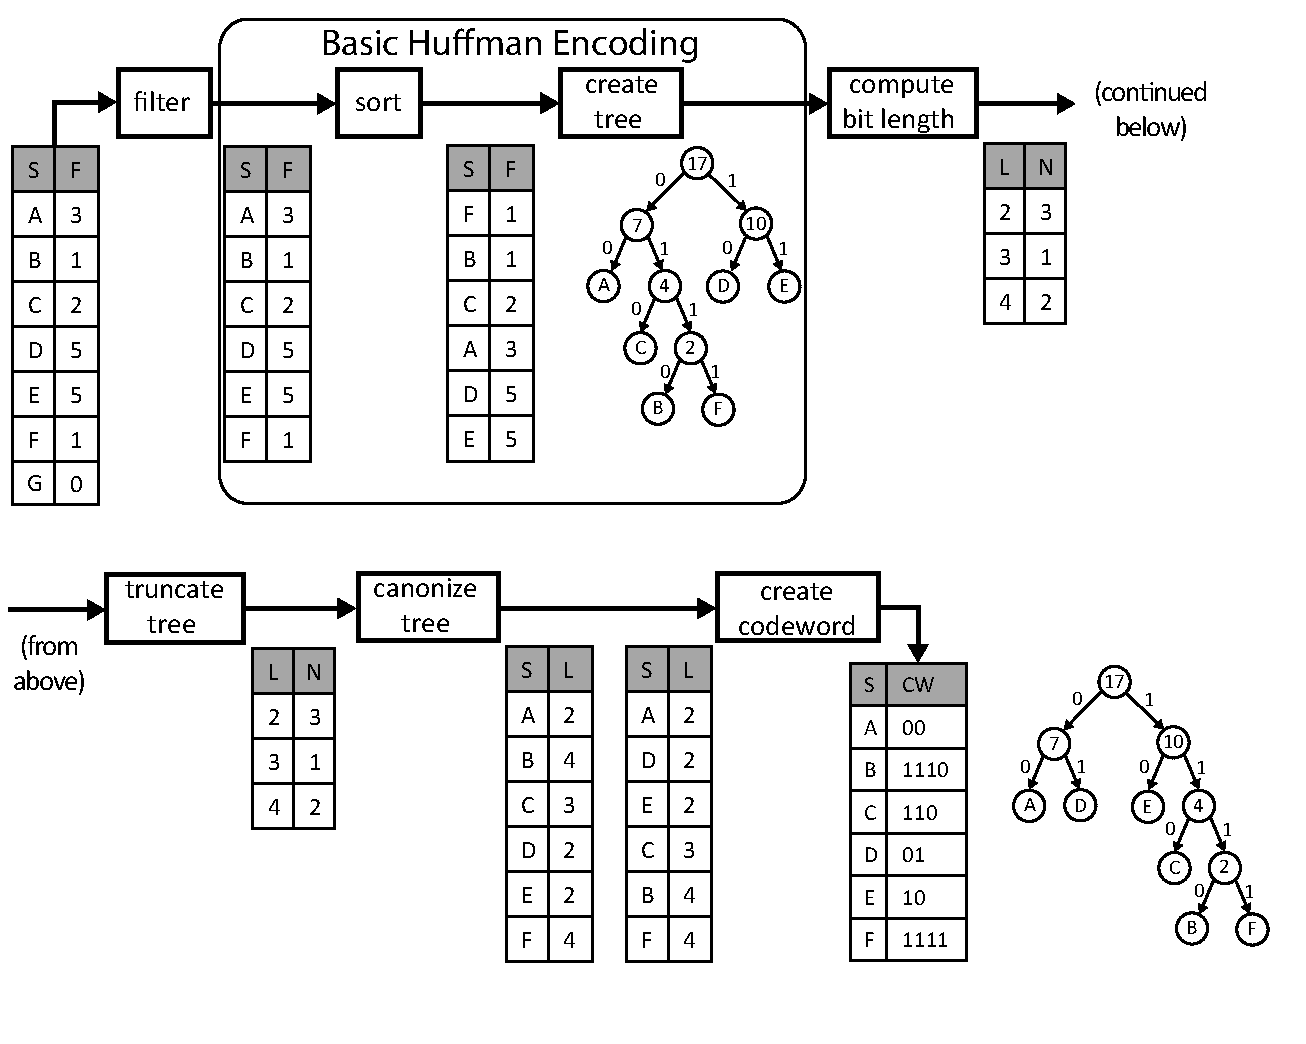
\includegraphics[width= \textwidth]{images/canonical_huffman_flow}
\caption{ The Canonical Huffman Encoding process. The symbols are filtered and sorted, and used to build a Huffman tree. Instead of passing the entire tree to the decoder (as is done in ``basic'' Huffman coding), the encoding is done such that only the length of the symbols in the tree is required by the decoder. Note that the final canonical tree is different from the initial tree created near the beginning of the process.}
\label{fig:canonical_huffman_flow}
\end{figure}

Figure~\ref{fig:canonical_huffman_flow} shows the process of creating a canonical Huffman code. The \lstinline{filter} module only passes symbols with non-zero frequencies. The \lstinline{sort} module rearranges the symbols in ascending order based upon their frequencies. Next, the \lstinline{create tree} module builds the Huffman tree using three steps: 1) it uses the two minimum frequency nodes as an initial sub-tree and generates a new parent node by summing their frequencies; 2) it adds the new intermediate node to the list and sorts them again; and 3) it selects the two minimum elements from the list and repeats these steps until one element remains. The result is a Huffman tree where each leaf node in the tree represents a symbol that can be coded and each internal node is labeled with the frequency of the nodes in that sub-tree.  By associating the left and right edges in the tree with bits $0$ and $1$, we can determine the unique codeword for each symbol based on the path to reach it from the root node. For example, the codeword for \sym{A} is $00$ and codeword for \sym{B} is $1110$. This completes the basic Huffman encoding process, but does not necessarily create the canonical Huffman tree.

To create the canonical Huffman tree, we perform several additional transformations.   First, the \lstinline{compute bit len} module calculates the bit length of each codeword and then counts the frequency of each length. The result is a histogram of the codeword lengths (see Section \ref{sec:histogram}).  In the example case, we have three symbols (\sym{A},\sym{D},\sym{E}) with the code length of 2. Therefore, the computed histogram maps contains value $3$ in location $2$. Next, the \lstinline{truncate tree} module rebalances the Huffman tree in order to avoid excessively long codewords. This can improve decoder speed at the cost of a slight increase in encoding time. This is not necessary in the example in Figure \ref{fig:canonical_huffman_flow}. We set the maximum height of the tree to 27.  Lastly, the \lstinline{canonize tree} module creates two sorted tables. The first table contains symbols and lengths sorted by symbol. The second table contains symbols and lengths sorted by lengths. These tables simplify the creation of the canonical Huffman codewords for each symbol.

The \lstinline{create codeword} module creates a table of canonical Huffman codewords by traversing the sorted tables. Beginning with the first codeword in the sorted table, it is assigned the all-zero codeword with the appropriate length.  Each following symbol with the same bit length is assigned the following codeword, which is formed by simply adding $1$ to the previous code word.  In our example, symbols \sym{A}, \sym{D}, and \sym{E} all have bit length $l = 2$ and are assigned the codewords $\sym{A} = 00$, $\sym{D} = 01$, and $\sym{E} = 10$.  Note that the symbols are considered in alphabetical order, which is necessary to make the tree canonical.  This process continues until we get to a codeword that requires a larger length, in which case we not only increment the previous codeword, but also shift left to generate a codeword of the correct length.  In the example, the next symbol is \sym{C} with a length of 3, which receives the codeword $\sym{C} = (10 + 1) << 1 = 11 << 1 = 110$. Continuing on, the next symbol is \sym{B} with a length of 4.  Once again we increment and shift by one. Thus the codeword for $\sym{B} = (110 + 1) << 1 = 1110$. The final codeword for symbol $\sym{F} = 1110 + 1 = 1111$. We explain this in more detail in Chapter \ref{sec:create_codewords}.  

%$for$ $l=K ~to ~1; Start[l]:=[Start[l+1]+N[l+1]]$ where $Start[l]$ is the starting canonical codeword for a length $l$, $K$ is the number of different code lengtshs, and $N[l]$ is the number of symbols with length $l$. In CHE, the first codeword for the symbol with the longest bit length starts all zeros. Therefore, the symbol $B$ is the first symbol with longest codeword so it is assigned $0000$. The next symbol with length 4 is $F$ and is assigned $0001$ by the second rule. The starting symbol for the next code length (next code length is 3) is calculated based on the first rule. The value is $Start[4] + N[4] = 0000 + 10 = 0010$. We drop any trailing $0$ yielding the codeworld for $C = 0001$. The remainder of they codewords are created in a similar manner.

The creation of a canonical Huffman code includes many complex and inherently sequential computations. For example, the \lstinline{create tree} module needs to track the correct order of the created sub trees, requiring careful memory management. Additionally, there is very limited parallelism that can be exploited. In the following, we discuss the hardware architecture and the implementation of the canonical Huffman encoding design using \VHLS. 

\begin{figure}
\lstinputlisting[format=none, lastline=43]{examples/huffman_encoding.cpp}
\end{figure}
\begin{figure}
\lstinputlisting[format=none,firstline=44]{examples/huffman_encoding.cpp}
\caption{  The ``top'' \lstinline{huffman_encoding} function. It defines the arrays and variables  between the various subfunctions.  These are described graphically in Figures \ref{fig:canonical_huffman_flow} and \ref{fig:che_dataflow}.  }
\label{fig:huffman_encoding.cpp}
\end{figure}

Figure \ref{fig:huffman_encoding.cpp} shows the entire ``top'' \lstinline{huffman_encoding} function. This sets up the arrays and other variables that are passed between the various subfunctions. And it instantiates these functions. 

There is some additional copying of data that may seem unnecessary. This is due to our use of the \lstinline{dataflow} directive. This imparts some restrictions on the flow of the variables between the subfunctions. In particular, there are some strict rules on producer and consumer relationships of data between the parts of the function. This requires that we replicate some of the data. For example, we create two copies of the arrays \lstinline{parent}, \lstinline{left} and \lstinline{right}. We also do the same with the array \lstinline{truncated_bit_length}. The former is done in a \lstinline{for} loop in the top \lstinline{huffman_encoding} function; the latter is done inside of the \lstinline{canonize_tree} function.

\begin{aside}
The \lstinline{dataflow} directive imposes restrictions on the flow of information in the function. Many of the restrictions enforce a strict producer and consumer relationship between the subfunctions.  One such restriction is that an array should be written to by only one function and it should be read by only one function. i.e., it should only serve as an output from one function and an input to another function. If multiple functions read from the same array, \VHLS will synthesize the code but will issue a warning and not use a dataflow pipelined architecture.  As a result, using dataflow mode often requires replicating data into multiple arrays. A similar problem occurs if a function attempts to read from and write to an array which is also accessed by another function.  In this case it is necessary to maintain an additional internal copy of the data inside the function.  We will discuss both of these requirements and how to adhere to them as we go through the code in the remainder of this chapter.
\end{aside}

\section{Implementation}
The canonical Huffman encoding process is naturally divided into subfunctions. Thus, we can work on each of these subfunctions on a one-by-one basis. Before we do that, we should consider the interface for each of these functions. 

Figure \ref{fig:che_dataflow} shows the functions and their input and output data. For the sake of simplicity, it only shows the interfaces with arrays, which, since they are large, we can assume are stored in block rams (BRAMs). Before we describe the functions and their inputs and outputs, we need to discuss the constants, custom data types, and the function interface that are defined in \lstinline{huffman.h}. Figure \ref{fig:huffman_h} shows the contents of this file. 

\begin{figure}
\lstinputlisting[lastline=40]{examples/huffman.h}
\caption{  The parameters, custom data type, and function interface for the top level function \lstinline{huffman_encoding}.  }
\label{fig:huffman_h}
\end{figure}

The \lstinline{INPUT_SYMBOL_SIZE} parameter specifies the maximum number of symbols that will be given as input for encoding.  In this case, we've set it to $256$, enabling the encoding of 8-bit ASCII data. The \lstinline{TREE_DEPTH} parameter specifies the upper bound for the length of an individual codeword during the initial Huffman tree generation. The \lstinline{CODEWORD_LENGTH} parameter specifies the target tree height when the Huffman tree is rebalanced in the function \lstinline{truncate_tree}. Finally, the \lstinline{CODEWORD_LENGTH_BITS} constant determines the number of bits required to encode a codeword length. This is equal to $\log_2 \lceil $\lstinline{CODEWORD_LENGTH}$\rceil$, which in this case is $5$.
% What are the tradeoffs in these parameters.
% show static computation of log2.

We create a custom data type \lstinline{Symbol} to hold the data corresponding the input values and their frequencies. This datatype is used in the \lstinline{filter}, \lstinline{sort}, and other functions in the encoding process that require access to such information. The data type has two fields \lstinline{value} and \lstinline{frequency}.  In this case we've assumed that the block of data being encoded contains no more than $2^{32}$ symbols.

Finally, the \lstinline{huffman.h} file has the \lstinline{huffman_encoding} function interface. This is the specified top level function for the \VHLS tool. It has three arguments. The first argument is an array of \lstinline{Symbols} of size \lstinline{INPUT_SYMBOL_SIZE}.  This array represents a histogram of the frequencies of the data in the block being encoded. The next two arguments are outputs. The \lstinline{encoding} argument outputs the codeword for each possible symbol. The \lstinline{num_nonzero_symbols} argument is the number of non-zero symbols from the input data. This is the same as the number of symbols that remain after the \lstinline{filter} operation. 

\begin{figure}
\centering
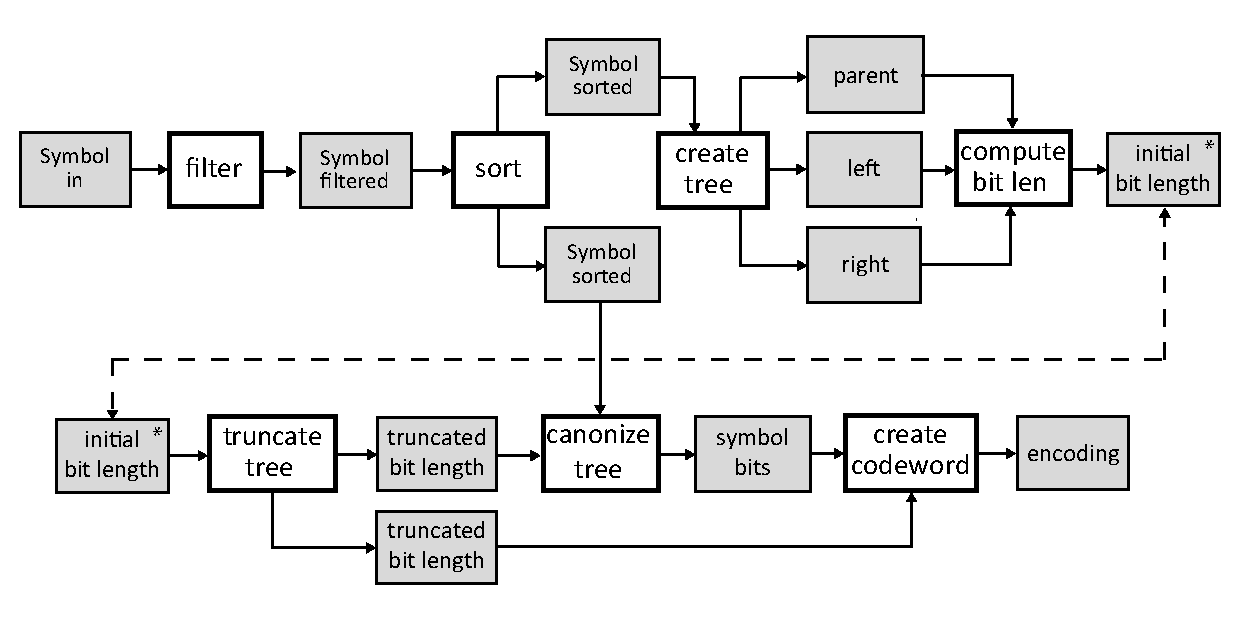
\includegraphics[width= \textwidth]{images/che_dataflow}
\caption{ The block diagram for our hardware implementation of canonical Huffman encoding. The gray blocks represent the significant input and output data that is generated and consumed by the different subfunctions. The white blocks correspond to the functions (computational cores). Note that the array initial bit length appears twice to allow the figure to be more clear.}
\label{fig:che_dataflow}
\end{figure}

%ugh.
The input to the system is an array of \lstinline{Symbol}. This holds the symbol value and frequencies in the array \lstinline{in}. Each symbol holds a 10-bit \lstinline{value} and a 32-bit \lstinline{frequency}. The size of this array is set as the constant \lstinline{INPUT_SYMBOL_SIZE} which is 256 in our example. The \lstinline{filter} module reads from the \lstinline{in} array and writes its output to the \lstinline{filtered} array. This is an array of \lstinline{Symbols} which holds the number of non-zero elements which is the input to the \lstinline{sort} module. The \lstinline{sort} module writes the symbols sorted by frequency into two different arrays -- one is used for the \lstinline{create tree} module and the other for the \lstinline{canonize tree} module. The \lstinline{create tree} module creates a Huffman tree from the sorted array and stores it into three arrays (\lstinline{parent}, \lstinline{left}, and \lstinline{right}); these arrays hold all the info for each node of the Huffman tree. Using the Huffman tree information, the \lstinline{compute bit len} module calculates the bit length of each symbol and stores this information to a \lstinline{initial bit len} array. We set the maximum number of entries to 64, covering up to maximum 64-bit frequency number, which is sufficient for most applications given that our Huffman tree creation rebalances its height. The \lstinline{truncate tree} module rebalances the tree height and copies the bit length information of each codeword into two separate \lstinline{truncated bit length} arrays. They each have the exact same information, but they must be copied to ensure that the \VHLS tool can perform functional pipelining; we will talk about that in more detail later. The \lstinline{canonize tree} module walks through each symbol from the \lstinline{sort} module and assigns the appropriate bit length using the \lstinline{truncated bit length} array. The output of the \lstinline{canonize} module is an array that contains the bit lengths for the codeword of each symbol. Finally, the \lstinline{create codeword} module generates the canonical codewords for each symbol.

\subsection{Filter}
 
The first function for the Huffman encoding process is \lstinline{filter}, which is shown in Figure \ref{fig:huffman_filter.cpp}. This function takes as input a \lstinline{Symbol} array. The output is another \lstinline{Symbol} array that is a subset of the input array \lstinline{in}. The \lstinline{filter} function removes any entry with a frequency equal to $0$.  The function itself simply iterates across the \lstinline{in} array, storing each element to the \lstinline{out} array if its \lstinline{frequency} field is non-zero. In addition, the function counts the number of non-zero entries to the output. This is passed as the output argument \lstinline{n}, enabling further functions to only process the `useful' data.

\begin{figure}
\lstinputlisting{examples/huffman_filter.cpp}
\caption{  The \lstinline{filter} function iterates across the input array \lstinline{in} and add any \lstinline{Symbol} entry with a non-zero \lstinline{frequency} field to the output array \lstinline{out}. Additionally, it records the number of non-zero frequency elements and passes that in the output argument \lstinline{n}.  }
\label{fig:huffman_filter.cpp}
\end{figure}

\begin{aside}
\VHLS can decide to automatically inline functions in order to generate a more efficient architecture. Most often, this happens for small functions.  The directive \lstinline{inline} allows the user to explicitly specify whether or not \VHLS should inline particular functions. In this case, \lstinline{INLINE off} ensures that this function will not be inlined and will appear as a module in the generated \gls{rtl} design. In this case, disabling inlining allows us to get a performance and resource usage for this function and to ensure that it will be implemented as a process in the toplevel dataflow design.
\end{aside}

%\begin{framed}
%\lstinputlisting[]{examples/huffman_sort.cpp}
%\captionof{figure}{some text}
%\label{fig:huffmanSort}
%\end{framed}

\begin{figure}
\lstinputlisting[format=none, lastline=39]{examples/huffman_sort.cpp}
\end{figure}
\begin{figure}
\lstinputlisting[format=none,firstline=40]{examples/huffman_sort.cpp}
\caption{  The \lstinline{sort} function employs a radix sort on the input symbols based upon their frequency values. }
\label{fig:huffman_sort.cpp}
\end{figure}

\subsection{Sort}

The \lstinline{sort} function, shown in Figure \ref{fig:huffman_sort.cpp}, orders the input symbols based on their \lstinline{frequency} values. The function itself consists of two \lstinline{for} loops, labeled \lstinline{copy_in_to_sorting} and \lstinline{radix_sort}. 

The \lstinline{copy_in_to_sorting} loop moves input data from the \lstinline{in} array into the \lstinline{sorting} array.  This ensures that the \lstinline{in} array is read-only to meet the requirements of the \lstinline{dataflow} directive used at the toplevel. The \lstinline{sorting} function reads and writes to the \lstinline{sorting} array throughout its execution. Even for simple loops like this, it is important to use the \lstinline{pipeline} directive to generate the most efficient result and accurate performance estimates.

The \lstinline{radix_sort} loop implements the core radix-sorting algorithm.   In general, radix sorting algorithms sort data by considering one digit or group of bits at a time.  The size of each digit determines the \term{radix} of the sort.  Our algorithm considers 4 bits at a time of the 32-bit \lstinline{Symbol.frequency} variable.  Hence we are using radix $r=2^{4}=16$ sort.  For each 4-bit digit in the 32-bit number, we perform a counting sort. The \lstinline{radix_sort} loop performs these 8 counting sort operations, iterating to $32$ in steps of $4$.   Radix-sorting algorithms can also operate from left to right (least significant digit first) or right to left (most significant digit first).   The algorithm implemented here works from least significant digit to most significant digit.   In the code, the radix can be configured by setting the \lstinline{RADIX} and \lstinline{BITS_PER_LOOP} parameters. 

\begin{exercise}
What would happen if we increased or decreased the radix? How would this effect the number of counting sort operations that are performed? How would this change the resource usage, e.g., the size of the arrays?
\end{exercise}

The code stores the current state of the sort in \lstinline{sorting[]} and \lstinline{previous_sorting[]}.  Each iteration of \lstinline{radix_sort_loop}, the current value of \lstinline{sorting[]} is copied to \lstinline{previous_sorting[]} and then the values are sorted as they are copied back into \lstinline{sorting[]}.  The \lstinline{digit_histogram[]} and \lstinline{digit_location[]} arrays are used in \lstinline{radix_sort_loop} to implement the counting sort on a particular digit. The two \lstinline{array_partition} s declare that these two arrays should be completely partitioned into registers. These arrays are small and used frequently, thus this does not use many resources and can provide performance benefits. Finally, \lstinline{current_digit[]} stores the digit being sorted for each item in the current iteration of the radix sort.

This code also contains two \lstinline{assert()} calls which check assumptions about the input \lstinline{num_symbols}.  Since this variable determines the number of valid elements in the \lstinline{in} array, it must be bounded by the size of that array.  Such assertions are good defensive programming practice in general to ensure that the assumptions of this function are met.  In \VHLS they serve an additional purpose as well.  Since \lstinline{num_symbols} determines the number of times that many of the internal loops execute, \VHLS can infer the tripcount of the loop based on these assertions.  In addition, \VHLS also uses these assertions to minimize the bitwidth of the variables used in the implemented circuit.

\begin{aside}
Previously we've seen the \lstinline{loop_tripcount} directive used to give \VHLS information about the tripcount of loops.   Using \lstinline{assert()} statements serves many of the same purposes, with some advantages and disadvantages.  One advantage of using \lstinline{assert()} statements is that they are checked during simulation and this information can be used to further optimize the circuit.  In contrast, the \lstinline{loop_tripcount} directive only affects performance analysis and is not used for optimization.  On the other hand, \lstinline{assert()} statements can only be used to give bounds on variable values, but can't be used to set expected or average values, which can only be done through the \lstinline{loop_tripcount} directive.  In most cases, it is recommended to first provide worst case bounds through \lstinline{assert()} statements, and then if necessary also add \lstinline{loop_tripcount} directives.
\end{aside}

The body of the \lstinline{radix_sort} loop is divided into four subloops, labeled \lstinline{init_histogram}, \lstinline{compute_histogram}, \lstinline{find_digit_location}, and \lstinline{re_sort}.  \lstinline{init_histogram} and \lstinline{compute_histogram} loops combine to compute the histogram of the input, based on the current digit being considered.  This produces a count of the number of each times each digit occurs in \lstinline{digit_histogram[]}.  The \lstinline{compute_histogram} loop also stores the current digit being sorted for each symbol in \lstinline{current_digit[]}.   Next, the \lstinline{find_digit_location} loop computes a prefix sum of the resulting histogram values, placing the result in \lstinline{digit_location[]}.  In the context of the counting sort, \lstinline{digit_location[]} contains the location of the first symbol with each digit in the newly sorted array.  Lastly, the \lstinline{re_sort} loop reorders the symbols based upon these results, placing each element in its correct place in the newly sorted array.    It uses the key stored in \lstinline{current_digit[]} to select the right location from \lstinline{digit_location[]}. This location is incremeted each time through the \lstinline{re_sort} loop to place the next element with the same digit in the next location in the sorted array.  Overall, each iteration through the \lstinline{radix_sort} loop implements a counting sort on one digit.  The counting sort is a \gls{stable_sort}, so that elements with the same digit remain in the same order.  After stable-sorting based on each digit, the array is returned in the correct final order.

We have previous discussed the histogram and prefix sum algorithms in Chapter \ref{sec:histogram} and \ref{sec:prefixSum}.  In this case, with simple code and complete partitioning of \lstinline{digit_histogram[]} and \lstinline{digit_location[]}, we can achieve a loop II of 1 to compute the histogram and prefix sum, since the number of bins is relatively small.  The optimization of the \lstinline{re_sort} loop is similar.  Since the only recurrence is through the relatively small \lstinline{digit_location[]} array, achieving a loop II of 1 is also straightforward.  Note that this approach works primarily because we've configured \lstinline{RADIX} to be relatively small.  With larger values of \lstinline{RADIX}, it would be preferable to implement \lstinline{digit_histogram[]} and \lstinline{digit_location[]} as memories, which might require additional optimization to achieve a loop II of 1.

Another alternative that may make sense in the context of this code is to combine complete partitioning of \lstinline{digit_histogram[]} and \lstinline{digit_location[]} with complete unrolling of the \lstinline{init_histogram} and \lstinline{find_digit_location} loops.   These loops access each location in these small arrays and perform operations with a minimal amount of logic.  In this case, although unrolling loops would likely result in replicating the circuit for each loop body, fewer resources would be required to implement this circuit since the array accesses would be at constant indexes.  However, for larger values of the \lstinline{BITS_PER_LOOP} parameter this change becomes prohibitive, since each additional bit doubles the \lstinline{RADIX} parameter, doubling the cost of these unrolled loops.  This is a somewhat common situation with parameterized code where different optimizations make sense with different parameter values.

\begin{exercise}
What happens to the performance and utilization results when you perform the optimizations on the prefix sum and histogram loops as specified in Chapter \ref{sec:histogram} and \ref{sec:prefixSum}?  Are these optimizations necessary in this case?
\end{exercise}

\begin{exercise}
Is the \lstinline{re_sort for} loop able to achieve the specified initiation interval of one cycle? Why or why not?
\end{exercise}

\begin{exercise}
For a large dataset ($n > 256$), what is the approximate latency, in terms of $n$, of the code in Figure \ref{fig:huffman_sort.cpp}.  What portions of the code dominate the number of cycles?  How would this change as the \lstinline{RADIX} parameter changes?
\end{exercise}

Note that the \lstinline{re_sort} loop not only stores the sorted arrray in \lstinline{sorting[]} but also stores the sorted array in \lstinline{out[]}.  While this may seem redundant, we need to ensure that \lstinline{out[]} is only written to in order to obey the requirements of the toplevel \lstinline{dataflow} directive.  In this case, \lstinline{out[]} will be overwritten multiple times with partially sorted results, but only the final result will be passed on the following function.

\begin{aside}
The \lstinline{dataflow} directive has several requirements in order to perform the task level pipelining optimization. One of them is the need for single producer and consumer of data between the tasks. Since we would like to perform task level pipelining for the Huffman encoding process as shown in Figure \ref{fig:che_dataflow}, we must insure that each of these tasks follow this requirement. In the case of this \lstinline{sort} function, which is one of the tasks, it must only consume (read from but not write to) the input argument data and only produce (write to but not read from) the output argument data. In order to met this requirement, we create the internal array \lstinline{sorting}, which is read from and written to throughout the function. We copy the input data from the argument \lstinline{in} at the beginning of the function and write the final results to the output argument \lstinline{out} at the end of the function. This insures that we follow the producer/consumer requirements for the \lstinline{dataflow} directive.
\end{aside}

\subsection{Create Tree}
The next function in the Huffman encoding process forms the binary tree representing the Huffman code. This is implemented in the \lstinline{create_tree} function shown in Figure \ref{fig:huffman_create_tree.cpp}. \lstinline{in[]} contains \lstinline{num_symbols} \lstinline{Symbol} elements, sorted from lowest to highest frequency. The function creates a binary tree of those symbols which is stored into three output arrays named \lstinline{parent}, \lstinline{left}, and \lstinline{right}.  The \lstinline{left} and \lstinline{right} arrays represent the left and right children of each intermediate node in the tree.  If the child is a leaf node, then the corresponding element of the \lstinline{left} or \lstinline{right} array will contain the symbol value of the child, otherwise it contains the special flag \lstinline{INTERNAL_NODE}.   Similarly, the \lstinline{parent} array holds the index of the parent node of each intermediate node.  The parent of the root node of the tree is defined to be index zero.  The tree is also ordered, in the sense that a parent  always has a higher index than its children.  As a result, we can efficiently implement bottom-up and top-down traversals of the tree. 

Figure \ref{fig:huffman_create_tree} shows an example of these data structures. Six symbols sorted by their frequencies are stored in the \lstinline{in} array. The resulting Huffman tree is stored in three arrays \lstinline{parent}, \lstinline{left}, and \lstinline{right}.  In addition, the frequency of each intermediate node is stored in the \lstinline{frequency} array.  We directly denote the node numbers for the \lstinline{left} and \lstinline{right} arrays (e.g., \lstinline{n0}, \lstinline{n1}, etc.) for the sake of illustration. These will hold a special internal node value in reality. 

\begin{aside}
While it may be odd to think of storing a complex data structure in a tree like this, it is actually very common in embedded programming where data allocation is not allowed\cite{misra2012}.  In fact, the C library implementations of \lstinline{malloc()} and \lstinline{free()} often implement low-level memory management in this way to enable small allocations to be created from larger memory allocations, usually called \term{pages}, returned from the operating system.  This enables the operating system to efficiently manage large allocations of memory efficiently and to coordinate virtual memory using the processor page table and disk storage which usually handle large blocks of data.  4 Kilo-bytes is a typical size for these pages.  For more ideas about implementing data structures using arrays, see \cite{sedgewickalgorithmsinC}.
\end{aside}

\begin{figure}
\centering
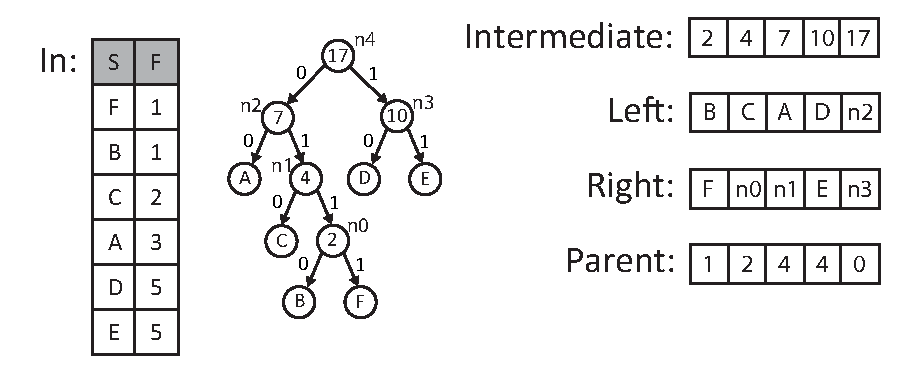
\includegraphics[width= \textwidth]{images/huffman_create_tree}
\caption{ The \lstinline{Symbol} array \lstinline{in} is used to create the Huffman tree. The tree is shown graphically along with the corresponding values for the four arrays used to represent the tree (\lstinline{intermediate}, \lstinline{left}, \lstinline{right}, and \lstinline{parent}).   }
\label{fig:huffman_create_tree}
\end{figure}

In the Huffman tree, each symbol is associated with a leaf node in the tree.  Intermediate nodes in the tree are created by grouping the two symbols with the smallest frequency and using them as the left and right nodes of a new intermediate node. That intermediate node has a frequency which is the sum of the frequencies of each child node. This process continues by iteratively creating intermediate nodes from the two nodes with the smallest frequencies, which may include other intermediate nodes or leaf nodes.  The tree building process completes when all of the intermediate nodes have been incorporated into the binary tree.

There are many ways to represent this process in code.  For instance, we might explicitly create an array representing every node in the tree which is sorted by frequency.  In this case selecting nodes to add to the tree is simple, since they will always be in the same locations of the sorted array.  On the other hand, inserting a newly created node into the list is relatively complex because the array must again be sorted, which would require moving elements around.  Alternatively, we might add pointer-like array indexes to the data structure in our array to enable the data to be logically sorted without actually moving the data around.  This would reduce data copying, but would increase the cost of accessing each element and require extra storage.  Many of the normal algorithmic tradeoffs in the design of data structures apply in the context of HLS just as well as they apply to processors.

In this case, however, we can make some additional simplifying observations.  The most important observation is that new intermediate nodes are always created in order of frequency.  We might create an intermediate node with a frequency that is less than the frequency of some leaf node, but we will never create an intermediate node with a frequency less than an already created intermediate node.  This suggests that we can maintain a sorted data structure by storing the nodes in two separate arrays: a sorted array of symbols and a sorted array of intermediate nodes.  As we `use' the lowest frequency elements of each list, we only need to append to the end of the list of intermediate nodes.  There is a small extra complexity because we might need to remove zero, one, or two elements from either array, but this turns out to be much less complex than resorting the node array.

\begin{aside}
Conceptually this algorithm is very similar to the mergesort algorithm discussed in Section \ref{sec:sort:merge}.   The key difference is what operation is done as elements are removed from the sorted arrays.  In mergesort, the least element is simply inserted at the appropriate position in the array.  In this case, the two least elements are identified and then merged into a new tree node.
\end{aside}
%This is an interesting function from an high-level synthesis standpoint since we simplify the data structures in order to make the resulting hardware less complex.  A typical implementation would use a queue or similar data structure in order to resort the nodes. That is, it would create a new intermediate node, and then add that back into the queue. And then take two elements from the queue, and continue this process until the queue is empty. However, this involves a lot of pointer chasing and/or array reordering. Instead, we use two arrays -- one that has a sorted list of the input symbols and one that keeps a sorted list of the intermediate nodes. This requires that we check each array for the lowest sorted values. Furthermore, we store the resulting tree into three arrays \lstinline{parent}, \lstinline{left}, and \lstinline{right}. These are used to store the nodes in the binary tree. Each index from the three arrays corresponds to one node. For example, \lstinline{parent[i]}, \lstinline{left[i]}, and \lstinline{right[i]} hold all of the information for the $i$th intermediate node of the binary tree (the parent of that node, and the left and right children respectively). These are stored in the order that they are created. Correspondingly, they are also stored in sorted order (based upon the frequency of their children) since the $i + 1$ intermediate node is guaranteed to have a frequency that is equal to or larger than node $i$. The frequency value for the node is stored at \lstinline{intermediate[i]}. 

\begin{figure}
\lstinputlisting[format=none, lastline=42]{examples/huffman_create_tree.cpp}
\end{figure}
\begin{figure}
\lstinputlisting[format=none, firstline=43, lastline=86]{examples/huffman_create_tree.cpp}
\end{figure}
\begin{figure}
\lstinputlisting[format=none, firstline=87]{examples/huffman_create_tree.cpp}
\caption{  The complete code for Huffman tree creation. The code takes as input the sorted \lstinline{Symbol} array \lstinline{in}, the number of elements in that array \lstinline{n}, and outputs the Huffman tree in the three arrays \lstinline{left}, \lstinline{right}, and \lstinline{parent}. }
\label{fig:huffman_create_tree.cpp}
\end{figure}

This code to implement the \lstinline{create_tree} function is shown in Figure \ref{fig:huffman_create_tree.cpp}.  The first block of code defines the local variables that we use in the function.  \lstinline{frequency[]} stores the frequencies for each intermediate node as it is created.   \lstinline{in_count} tracks which symbols have been given a parent node in the tree, while \lstinline{tree_count} tracks which newly created intermediate nodes have been given a parent node.  Each iteration through the main loop creates a new intermediate node without a parent, so all of the intermediate nodes between \lstinline{tree_count} and \lstinline{i} have not yet been assigned a parent in the tree.

The main loop contains two similar blocks of code.  Each block compares the frequency of the next available symbol \lstinline{in[in_count].frequency} with the frequency of the next available intermediate node \lstinline{frequency[tree_count]}.  It then selects the lowest frequency of the two to be incorporated as the leaf of a new intermediate node.  The first block does this for the left child of the new node, storing in \lstinline{left[i]}, while the second block selects the right child of the new node, storing in \lstinline{right[i]}.  In both cases, we need to be careful to ensure that the comparison is meaningful.  In the first iteration of the loop, \lstinline{tree_count == 0} and \lstinline{i == 0}, so there is no valid intermediate node to be considered and we must always select an input symbol.  During the final iterations of the loop, it is likely that all of the input symbols will have been consumed, so \lstinline{in_count == num_symbols} and we must always consume an intermediate node.

The number of iterations of the loop depends on the input \lstinline{num_symbols} in an interesting way.  Since each input symbol becomes a leaf node in the binary tree, we know that there will be exactly \lstinline{num_symbols-1} intermediate nodes to be created, since this is a basic property of a binary tree.  At the end of the loop we will have created \lstinline{num_symbols-1} new nodes, each of which has two children. \lstinline{num_symbols} of these children will be input symbols and \lstinline{num_symbols-2} will be intermediate nodes.  There will be one intermediate node remaining as the root of the tree without a parent.  This last node is artificially assigned a parent index of zero in the last line of code.  This completes the building of the Huffman tree.

In the tree, the children of an intermediate node can be either a symbol or a intermediate node.  In creating the huffman tree, this information isn't very important, although it will be important later when we traverse the tree later.  To store this difference
a special value \lstinline{INTERNAL_NODE} is stored in \lstinline{left[]} and \lstinline{right[]} if the corresponding child is an internal node.   Note that this storage essentially requires one more bit to represent in the array.  As a result, the \lstinline{left[]} and \lstinline{right[]} arrays are one bit larger than you might expect. 



\begin{exercise}
For a large dataset ($n > 256$), what is the approximate latency, in terms of $n$, of the code in Figure \ref{fig:huffman_create_tree.cpp}?  What portions of the code dominate the number of cycles?
\end{exercise}

\subsection{Compute Bit Length}

The \lstinline{compute_bit_length} function determines the depth in the tree for each symbol.  The depth is important because it determines the number of bits used to encode each symbol. Computing the depth of each node in the tree is done using the recurrence:
\begin{equation}
\begin{array}{rrcl}
&\mathrm{depth}(\mathrm{root}) &=& 0 \\
\forall n != \mathrm{root}, &\mathrm{depth}(n) &=& \mathrm{depth}(\mathrm{parent}(n)+1)\\
\forall n, &\mathrm{child\_depth}(n) &=& \mathrm{depth}(n)+1
\end{array}
\end{equation}

This recurrence can be computed by traversing the tree starting at the root node and exploring each internal node in order.  As we traverse each internal node, we can compute the depth of the node and the corresponding depth (incremented by one) of any child nodes.  It turns out that we don't actually care about the depth of the internal nodes, only about the depth of the child nodes.  As a result, the code actually computes the recurrence:
\begin{equation}
\begin{array}{rrcl}
&\mathrm{child\_depth}(\mathrm{root}) &=& 1 \\
\forall n != \mathrm{root}, &\mathrm{child\_depth}(n) &=& \mathrm{child\_depth}(\mathrm{parent}(n)+1)
\end{array}
\end{equation}

The code for this function is shown in Figure \ref{fig:huffman_compute_bit_length.cpp}.  The input arguments to the function represent a Huffman tree in \lstinline{parent[]}, \lstinline{left[]}, and \lstinline{right[]}.   \lstinline{num_symbols} contains the number of input symbols, which is one more than the number of intermediate nodes in the tree.  The output \lstinline{length_histogram[]}.  Each element of that array stores the number of symbols with the given depth. Thus, if there are five symbols with depth three, then \lstinline{length_histogram[3] = 5}. 
\begin{figure}
\lstinputlisting[format=none]{examples/huffman_compute_bit_length.cpp}
\caption{The complete code for determining the number of symbols at each bit length.}
\label{fig:huffman_compute_bit_length.cpp}
\end{figure}

\lstinline{child_depth[]} stores the depth of each internal node while the tree is being traversed.  After the depth of each internal node is determined in the \lstinline{traverse_tree} loop, \lstinline{length_histogram[]} is updated.  \lstinline{internal_length_histogram[]} is used to ensure that our function adheres the requirements for the \lstinline{dataflow} directive, where the output array \lstinline{length_histogram[]} is never read.  The \lstinline{init_histogram} loop initializes these two arrays.

\begin{exercise}
The \lstinline{init_histogram} loop has a \lstinline{pipeline} directive with \lstinline{II = 1}. Is it possible to meet this II? What happens if we increase the II to something larger? What happens if we do not apply this directive?
\end{exercise}

Internal nodes in the tree are traversed from the root node, which has the largest index, down to index zero.  Since the array of nodes were created in bottom-up order, this reverse order results in a top-down traversal of the tree enabling the computation of the recurrence for each node in a single pass through the nodes.  For each node, we determine the depth of its children.  Then if the node actually does have any children which are symbols, we figure out how many children and update the histogram accordingly.  Child nodes which are internal nodes are represented by the special value \lstinline{INTERNAL_NODE}.

\begin{exercise}
For a large dataset ($n > 256$), what is the approximate latency, in terms of $n$, of the code in Figure \ref{fig:huffman_compute_bit_length.cpp}?  What portions of the code dominate the number of cycles?
\end{exercise}

\begin{exercise}
This code has several recurrences.  For example, one recurrence occurs because of the histogram computation.  In this case, the loop is synthesized with an II of 3.  What happens if you target a lower II in the \lstinline{pipeline} directive?  Can you rewrite the code to eliminate the recurrences and achieve a lower II?
\end{exercise}

\subsection{Truncate Tree}
\label{sec:huffman_truncate_tree}

The next part of the Huffman encoding process reorganizes nodes with a depth that is larger than that specified in \lstinline{MAX_CODEWORD_LENGTH}. This is done by finding any symbols with a greater depth, and moving them to a level that is smaller than that specified target.   Interestingly, this can be done entirely by manipulating the histogram of symbol depths, as long as the histogram is modified in a way that is consistent with the same modifications on the original tree.

% more depth here would be good.

The input histogram is contained in \lstinline{input_length_histogram}, which was derived by the \lstinline{compute_bit_length()} function described in the previous section. There are two identical output arrays \lstinline{truncated_length_histogram1} and \lstinline{truncated_length_histogram2}. These arrays are passed to two separate functions later in the process (\lstinline{canonize_tree} and \lstinline{create_codewords}), and thus we must have two arrays to adhere to the single producer, single consumer constraint of the \lstinline{dataflow} directive.

\begin{figure}
\lstinputlisting[lastline=39]{examples/huffman_truncate_tree.cpp}
\end{figure}
\begin{figure}
\lstinputlisting[format=none, firstline=40]{examples/huffman_truncate_tree.cpp}
\caption{The complete code for rearranging the Huffman tree such that the depth of any node is under the target specified by the parameter \lstinline{MAX_CODEWORD_LENGTH}. }
\label{fig:huffman_truncate_tree.cpp}
\end{figure}

The code is shown in Figure \ref{fig:huffman_truncate_tree.cpp}. The \lstinline{copy_input} loop copies the data from the input array \lstinline{input_length_histogram}. The \lstinline{move_nodes} loop contains the bulk of the processing to modify the histogram.  Lastly, the \lstinline{input_length_histogram} function copies the internal result to other output at the end of the function. 

\begin{exercise}
The \lstinline{copy_in for} loop is not optimized. What happens to the latency and initiation interval of the \lstinline{truncate_tree} function if we use a \lstinline{pipeline} or \lstinline{unroll} directive on this loop. What happens to the overall latency and initiation interval of the design (i.e., the \lstinline{huffman_encoding} function)?
\end{exercise}

The function continues in the second \lstinline{move_nodes for} loop, which performs the bulk of the computation. This \lstinline{for} loop starts by iterating through the \lstinline{truncated_length_histogram} array from the largest index (\lstinline{TREE_DEPTH} - the specified maximum depth for a tree). This continues down through the array until there is a non-zero element or \lstinline{i} reaches the \lstinline{MAX_CODEWORD_LENGTH}. If we do not find a non-zero element, that means the initial input Huffman tree does not have any nodes with a depth larger than the target depth. In other words, we can exit this function without performing any truncation. If there is a value larger than the target depth, then the function continues by reorganizing the tree so that all of the nodes have depth smaller than the target depth. This is done by the operations in the \lstinline{reorder while} loop. When there are nodes to move, the \lstinline{move_nodes for} loop goes through them from those with the largest depth, and continues to smaller depths until all nodes are rearranged with a depth smaller than the target. Each iteration of this \lstinline{move_nodes for} loops works on moving nodes from one depth at a time.

The \lstinline{reorder while} loop moves one node in each iteration. The first \lstinline{if} statement is used to find the leaf node with the largest depth. We will then alter this node by making it an intermediate node, and adding it and the leaf node with a depth larger than than target as children. This \lstinline{if} clause has a \lstinline{do/while} loop that iterates downward from the target looking for a non-zero entry in the \lstinline{truncated_length_histogram} array. It works in a similar manner as the beginning of the \lstinline{move_nodes for} loop. When it has found the deepest leaf node less than the target depth, it stops. The depth of this node is stored in \lstinline{j}.

Now we have a node with a depth \lstinline{i} larger than the target, and a node with a depth smaller than the target stored in \lstinline{j}. We move the node from depth \lstinline{i} and a node from \lstinline{j} into child nodes at depth \lstinline{j + 1}. Therefore, we add two symbols to \lstinline{truncated_length_histogram[j+1]}. We are making a new intermediate node a depth \lstinline{j} thus, we subtract a symbol from that level. We move the other leaf node from depth \lstinline{i} to depth \lstinline{i - 1}. And we subtract two from \lstinline{truncated_length_histogram[i]} since one of the nodes went to level \lstinline{j + 1} and the other when to level \lstinline{i - 1}. These operations are performed in the four statements on the array \lstinline{truncated_length_histogram}. Since we added a symbol to level \lstinline{j + 1}, we update \lstinline{j}, which holds the highest level under the target level, and then we repeat the procedure. This is done until there are no additional symbols with a depth larger than the target.

The function completes by creating an additional copy of the new bit lengths. This is done by storing the updated bit lengths in the array \lstinline{truncated_length_histogram1} into the array \lstinline{truncated_length_histogram2}. We will pass these two arrays to the final two functions in the \lstinline{huffman_encoding} top function; we need two arrays to insure that the constraints of the \lstinline{dataflow} directive are met.

\subsection{Canonize Tree}
\label{sec:huffman_canonize_tree}

The next step in the encoding process is to determine the number of bits for each of the symbols. We do this in the \lstinline{canonize_tree} function shown in Figure \ref{fig:huffman_canonize_tree.cpp}. The function takes as input an array of symbols in sorted order, the total number of symbols (\lstinline{num_symbols}), and a histogram of lengths describing the Huffman tree. The output \lstinline{symbol_bits[]} contains the number of encoded bits used for each symbol. Thus, if the symbol with value \lstinline{0x0A} is encoded in 4 bits, then \lstinline{symbol_bits[10] = 4}. 

\begin{figure}
\lstinputlisting[firstline=1]{examples/huffman_canonize_tree.cpp}
\caption{ The complete code for canonizing the Huffman tree, which determins the number of bits for each symbol. }
\label{fig:huffman_canonize_tree.cpp}
\end{figure}

The canonization process consists of two loops, labeled \lstinline{init_bits} and \lstinline{process_symbols}.  The \lstinline{init_bits} loop executes first, initializing \lstinline{symbol_bits[]} array to \lstinline{0}. The \lstinline{process_symbols} loop then processes the symbols in sorted order from smallest frequency to largest frequency. Naturally, the least frequent symbols are assigned the longest codes while the most frequent symbols are assigned the shortest code.  Each time through the \lstinline{process_symbols} loop, we assign the length of one symbol.  The length of the symbol is determined by the the inner \lstinline{do/while} loop, which steps through the histogram of lengths. This loop finds the largest bit length that has not yet had codewords assigned and stores the number of codewords in that length in \lstinline{count}. Each time through the outer loop, \lstinline{count} is decremented until we run out of codewords.  When \lstinline{count} becomes zero, the inner \lstinline{do/while} loop executes again to find a length with codewords to assign.

\begin{figure}
\lstinputlisting{examples/huffman_canonize_tree_alternate.cpp}
\caption{ Alternate loop structure for the \lstinline{process_symbols} loop in Figure \ref{fig:huffman_canonize_tree.cpp}. }
\label{fig:huffman_canonize_alternate}
\end{figure}

Note that the \lstinline{process_symbols} loop cannot be pipelined because the inner \lstinline{do/while} loop cannot be unrolled.  This is somewhat awkward as the inner loop will usually execute exactly once, stepping to the next length in the histogram.  Only in somewhat rare cases will the inner loop need to execute more than once if we happen to get to a length which does not have any codewords assigned.  In this case, there's not too much of a loss since all the operations in the loop are simple operations that are unlikely to be pipelined, with the exception of the memory operations.  There are other ways to structure this loop, however, which {\em can} be pipelined.  One possibility is to use an outer \lstinline{for} loop to iterate over \lstinline{codeword_length_histogram[]} and an inner loop to count each symbol, as shown in Figure \ref{fig:huffman_canonize_alternate}.

\begin{exercise}
Implement the code in Figure \ref{fig:huffman_canonize_tree.cpp} and the alternate code structure in Figure \ref{fig:huffman_canonize_alternate}.  Which results in higher performance?  Which coding style is more natural to you?
\end{exercise}

\subsection{Create Codeword}
\label{sec:create_codewords}

The final step in the encoding process is to create the codeword for each symbol.  This process simply assigns each symbol in order according to the properties of a Canonical Huffman code.  The first property is that longer length codes have a higher numeric value than the same length prefix of shorter codes.  The second property is that codes with the same length increase by one as the symbol value increases.  In order to achieve these properties while keeping the code simple, it is useful to determine the first codeword of each length.  If we know the number of codewords of each length given by $\mathrm{codeword\_length\_histogram}$, then this can be found using the following recurrence:
\begin{equation}
\begin{array} {rrcl}
&\mathrm{first\_codeword}(1) &=& 0 \\
\forall i > 1, &\mathrm{first\_codeword}(i) &=& (\mathrm{first\_codeword}(i-1) + \mathrm{codeword\_length\_histogram}(i-1)) << 1
\label{eq:first_codeword_recurrence}
\end{array}
\end{equation}  
Essentially, rather than actually assigning the codewords one after another, this recurrence allocates all the codewords first.  This allows us to actually assign the codewords in order of symbol value without being concerned about also ordering them by length or frequency.

In addition to assigning codewords to symbols, we also need to format the codewords so that they can be easily used for encoding and decoding.  Systems that use Huffman encoding often store codewords in bit-reversed order. This can make the decoding process easier since the bits are stored in the same order that the tree is traversed during decoding, from root node to leaf node. 

The code implementing the \lstinline{create_codewords} function is shown in Figure \ref{fig:huffman_create_codeword.cpp}. \lstinline{symbol_bits[]} contains the length of the codeword for each symbol and \lstinline{codeword_length_histogram[]} contains the number of codewords with each length. The output \lstinline{encoding[]} represents the encoding for each symbol. Each element consists of the actual codeword and the length of each codeword packed together.  The maximum length of a codeword is given by the \lstinline{MAX_CODEWORD_LENGTH} parameter.  In turn, this determines the number of bits required to hold the codeword, which is given by  \lstinline{CODEWORD_LENGTH_BITS}. The \lstinline{CODEWORD_LENGTH_BITS} least significant bits of each element in the \lstinline{encoding} array contains the same value received from the input array \lstinline{symbol_bits}. The high order \lstinline{MAX_CODEWORD_LENGTH} bits of each \lstinline{encoding} element contains the actual codeword.  Using 27 bits for \lstinline{MAX_CODEWORD_LENGTH} resulting in \lstinline{CODEWORD_LENGTH_BITS} of 5 is a particularly useful combination, since each element of \lstinline{encoding[]} fits in a single 32-bit word.

The code consists primarily of two loops, labeled \lstinline{first_codewords} and \lstinline{assign_codewords}.  The \lstinline{first_codewords} loop finds the first codeword with each length, implementing the recurrence in Equation \ref{eq:first_codeword_recurrence}.   The \lstinline{assign_codewords} loop finally associates each symbol with a codeword.  The codeword is found using the length of each codeword and indexing into the correct element of \lstinline{first_codeword[]}.  The main complexity of this code is in the bit reversal process, which is based on the \lstinline{bit_reverse32} function. We have talked about this function previously in the FFT chapter (see Chapter \ref{sec:fft_bit_reversal}), so we will not discuss it here again. After reversing the bits in the codeword, the next statement removes the least significant '0' bits leaving only the bit-reversed codeword. The bit-reversed codeword is then packed in the high-order bits together with the length of the symbol in the low-order bits and stored in \lstinline{encoding[]}.  Lastly, the value in \lstinline{first_codeword[]} is incremented.

\begin{figure}
\lstinputlisting[firstline=1]{examples/huffman_create_codeword.cpp}
\caption{ The complete code for generating the canonical Huffman codewords for each of the symbols. The codewords can be computed with knowledge of number of bits that each symbol uses (stored in the input array \lstinline{symbol_bits[]}). Additionally, we have another input array \lstinline{codeword_length_histogram[]} which stores at each entry the number of symbols with codewords at that bit length. The output is the code word for each symbol stored in the \lstinline{encoding[]} array. }
\label{fig:huffman_create_codeword.cpp}
\end{figure}

\begin{exercise}
In the code in Figure \ref{fig:huffman_create_codeword.cpp}, the inputs actually contain some redundant information.  In particular, we could compute the number of symbols for each bit length stored in \lstinline{codeword_length_histogram[]} from the length of each codeword \lstinline{symbol_bits[]} using a histogram computation.  Instead, in this code we've chosen to reuse the histogram originally computed in the \lstinline{truncate_tree()} function.  Instead we could save the storage by recomputing the histogram.  Do you think this is a good tradeoff?   How many resources are required to compute the histogram in this function?  How many resources are required to communicate the histogram through the pipeline?
\end{exercise}

\begin{exercise}
Estimate the latency of the code in Figure \ref{fig:huffman_create_codeword.cpp}
\end{exercise}

Let us now go through our running example and show how this is used to derive the initial codewords. In the example, the symbols \sym{A}, \sym{D}, and \sym{E} have two bits for their encoding; symbol \sym{C} has three bits; and symbols \sym{B} and \sym{F} have four bits. Thus, we have:
\begin{equation}
\begin{array} {lcl} 
\mathrm{bit\_length}(1) & = & 0 \\
\mathrm{bit\_length}(2) & = & 3 \\
\mathrm{bit\_length}(3) & = & 1 \\
\mathrm{bit\_length}(4) & = & 2 \\
\end{array}
\label{eq:bit_lengths}
\end{equation}

Using Equation \ref{eq:first_codeword_recurrence} to calculate the values of \lstinline{first_codeword}, we determine:
\begin{equation}
\begin{array} {lllll} 
\mathrm{first\_codeword}(1) & = & 0 & = & \mathrm{0b0}\\
\mathrm{first\_codeword}(2) & = & (0 + 0) << 1 &=& \mathrm{0b00} \\
\mathrm{first\_codeword}(3) & = & (0 + 3) << 1 &=& 6 = \mathrm{0b110} \\
\mathrm{first\_codeword}(4) & = & (6 + 1) << 1 &=& 14 = \mathrm{0b1110} \\
\end{array}
\label{eq:symbols}
\end{equation}

Once we have determined these values, then consider each symbol in order from smallest to largest. For each symbol, we determine the length of its codeword and assign the next codeword of the appropriate length.  In the running example, we consider symbols \sym{A}, \sym{B}, \sym{C}, \sym{D}, \sym{E}, and \sym{F} in alphabetical order. The symbol \sym{A} has two bits for its encoding. We perform a lookup into \lstinline{first_codeword[2] = 0}. Thus we assign the codeword for \sym{A} to \lstinline{0b00}. We increment the value at \lstinline{first_codeword[2]} to $1$. The symbol \sym{B} has four bits. Since \lstinline{first_codeword[4] = 14 = 0b1110}, it gets assigned the codeword \lstinline{0b1110}. Symbol \sym{C} has three bits. The value of \lstinline{first_codeword[3] = 6 = 0b110}, thus it gets the codeword \lstinline{110}. Symbol \sym{D} has two bits so it gets \lstinline{first_codeword[2] = 1 = 0b01}; remember that we incremented this value after we assigned the codeword to symbol \sym{A}. Symbol \sym{E} has two bits so it gets the codeword \lstinline{0b01 + 1 = 0b10}. And F has four bits so it gets the codeword \lstinline{0b1110 + 1 = 0b1111}.

The final codewords for all of the symbols are:
\begin{equation}
\begin{array} {lll} 
\sym{A} & \rightarrow & 00 \\
\sym{B} & \rightarrow & 1110\\
\sym{C} & \rightarrow  & 110 \\
\sym{D} & \rightarrow & 01 \\
\sym{E} & \rightarrow & 10\\
\sym{F} & \rightarrow & 1111\\
\end{array}
\label{eq:codewords}
\end{equation}

\subsection{Testbench}
\label{sec:huffman_testbench}

The final part of the code is the testbench. This is shown in Figure \ref{fig:huffman_encoding_test.cpp}. The general structure is to read the input frequency values from a file, process them using the \lstinline{huffman_encoding} function, and compare the resulting codewords with an existing golden reference that is stored in a file. 

\begin{figure}
\lstinputlisting[format=none, firstline=1,lastline=42]{examples/huffman_encoding_test.cpp}
\end{figure}
\begin{figure}
\lstinputlisting[format=none, firstline=43]{examples/huffman_encoding_test.cpp}
\caption{ The complete code for the canonical Huffman encoding testbench. The code initializes the \lstinline{in} array with data from an input file. It passes that into the top \lstinline{huffman_encoding} function. Then it stores the resulting codewords into a file, and compares that with another golden reference file. It prints out the results of the comparison, and returns the appropriate value.}
\label{fig:huffman_encoding_test.cpp}
\end{figure}

The \lstinline{main()} function starts by setting up the variables required to read the frequencies from a file (in this case the file is \texttt{huffman.random256.txt}) and puts them into \lstinline{in[]}. This is done in the \lstinline{file_to_array} function, which takes as input the \lstinline{filename} for the input data and the length of the data (\lstinline{array_length}), and stores the entries in that file into \lstinline{array[]} variable. This file contains the frequency of each symbol. Frequency values are stored in symbol order, thus the first value of the file represents the frequency of symbol '0', and so on. 

The \lstinline{main()} function continues by initializing \lstinline{in[]} using the frequencies from the file. It then calls the top \lstinline{huffman_encoding} function. The function returns the encoded symbol values in \lstinline{encoding[]}. Since the result of processing should be a prefix code, we check that the properties of a prefix code are actually satisfied.  The result is then compared to the codewords stored in a golden reference, which is stored in the file \texttt{huffman.random256.gold}. We do this by writing the result to a file named \texttt{random256.out} and performing a file comparison using the \texttt{diff} tool. The \texttt{diff} tool returns '0' if the files are identical and non-zero if the files are different. Thus, the \lstinline{if} condition occurs when the files are different, and the \lstinline{else} condition is executed when the files are the same. In both cases, we print out a message and set the \lstinline{return_val} to the appropriate value. This return value is used by the \VHLS tool during cosimulation to check the correctness of results.  The return value should be '0' if it passes, and non-zero if it does not pass.

\section{Conclusion}

Huffman Coding is a common type of data compression used in many applications.  While encoding and decoding using a Huffman code are relatively simple operations, generating the Huffman code itself can be a computationally challenging problem.  In many systems it is advantageous to have relatively small blocks of data, implying that new Huffman codes must be created often, making it worthwhile to accelerate.

Compared to other algorithms we've studied in this book, creating a Huffman code contains a number of steps with radically different code structures.  Some are relatively easy to parallelize, while others are more challenging.  Some portions of the algorithm naturally have higher $\mathcal{O}(n)$ complexity, meaning that they must be more heavily parallelized to achieve a balanced pipeline.  However, using the \lstinline{dataflow} directive in \VHLS, these different code structures can be linked together relatively easily